\documentclass[../../main.tex]{subfiles}
\begin{document}

\begin{flushright}
  \footnotesize\textit{【自動文字起こし・要確認】}
\end{flushright}

{\bf [解答]} 点 $\text{X}$ に対し，$\overrightarrow{\text{OX}} = \vec{x}$ と定めると，

$\vec{a}, \vec{b}, \vec{c}$ は1次独立 $\cdots \text{①}$．題意から
\begin{align}
  \begin{cases}
    \vec{p} = p\vec{a} \\
    \vec{q} = q\vec{a} + (1-q)\vec{b} \\
    \vec{r} = r\vec{b} + (1-r)\vec{c} \\
    \vec{s} = s\vec{c}
  \end{cases}
\end{align}
とおける．$p \sim s$ はいずれも $0 < p,q,r,s < 1$ をみたす実数．

\begin{figure}[H]
  \centering
  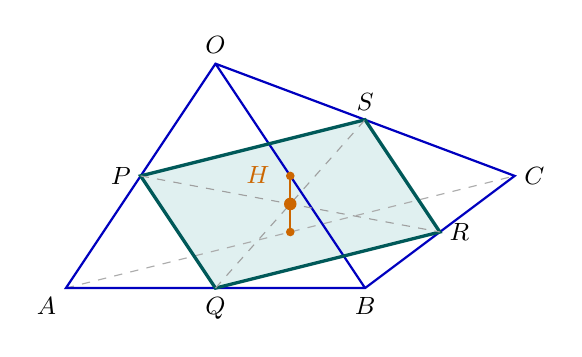
\begin{tikzpicture}[scale=0.95,every node/.style={font=\small}]
    % p=q=s=1/2, r=1/2 の例．H は PR と QS の共通中点．
    \coordinate (O) at (0,3);
    \coordinate (A) at (-2,0);
    \coordinate (B) at (2,0);
    \coordinate (C) at (4,1.5);
    \coordinate (P) at (-1,1.5);
    \coordinate (Q) at (0,0);
    \coordinate (R) at (3,0.75);
    \coordinate (S) at (2,2.25);
    \coordinate (M) at (1,0.75);
    \coordinate (N) at (1,1.5);
    \coordinate (H) at (1,1.125);
    \fill[teal!12] (P)--(Q)--(R)--(S)--cycle;
    \draw[gray!65,dashed] (A)--(C);
    \draw[blue!75!black,thick] (O)--(A)--(B)--(C)--cycle (O)--(B);
    \draw[teal!70!black,very thick] (P)--(Q)--(R)--(S)--cycle;
    \draw[gray!75,dashed] (P)--(R) (Q)--(S);
    \draw[orange!80!black,thick] (M)--(N);
    \node[circle, fill=orange!80!black, inner sep=1.1pt] at (M) {}; \node[circle, fill=orange!80!black, inner sep=1.1pt] at (N) {}; \node[circle, fill=orange!80!black, inner sep=1.6pt] at (H) {};
    \node[above] at (O) {$O$};
    \node[below left] at (A) {$A$};
    \node[below] at (B) {$B$};
    \node[right] at (C) {$C$};
    \node[left] at (P) {$P$};
    \node[below] at (Q) {$Q$};
    \node[right] at (R) {$R$};
    \node[above] at (S) {$S$};
    \node[above left=4pt,orange!80!black] at (H) {$H$};
  \end{tikzpicture}
  \caption{平行四辺形$PQRS$の対角線の交点$H$と，$AC$・$OB$の中点を結ぶ線分}
\end{figure}

\begin{align}
  \begin{cases}
    \overrightarrow{\text{PQ}} = (q-p)\vec{a} + (1-q)\vec{b} \equiv \vec{A} \\
    \overrightarrow{\text{PS}} = -p\vec{a} + s\vec{c} \equiv \vec{B} \\
    \overrightarrow{\text{PR}} = -p\vec{a} + r\vec{b} + (1-r)\vec{c}
  \end{cases} \quad \cdots *
\end{align}
\begin{align}
  \overrightarrow{\text{PH}} = \dfrac{1}{2}\overrightarrow{\text{PR}} = \dfrac{1}{2}(\overrightarrow{\text{PS}} + \overrightarrow{\text{PQ}}) \quad ( \text{HはPR, SQの中点} ) \quad \cdots \text{②}
\end{align}
\begin{align}
  \quad \overrightarrow{\text{PR}} = \vec{A} + \vec{B}
\end{align}

$*$を代入して
\begin{align}
  \quad -p\vec{a} + r\vec{b} + (1-r)\vec{c} = (q-2p)\vec{a} + (1-q)\vec{b} + s\vec{c}
\end{align}

①から
\begin{align}
  \begin{cases}
    -p = q-2p \\
    r = 1-q \\
    1-r = s
  \end{cases}
  \quad \therefore
  \begin{cases}
    q = s = p \\
    r = 1-p
  \end{cases}
\end{align}

②に代入して
\begin{align}
  \quad \vec{h} = \dfrac{1}{2}( p\vec{a} + (1-p)\vec{b} + p\vec{c} ) \quad \cdots \text{③}
\end{align}

一方，題意の線分上の点 $\text{X}$ は $\gamma$ に対して $(0 < \gamma < 1)$
\begin{align}
  \quad \vec{x} = \gamma \dfrac{\vec{a}+\vec{c}}{2} + (1-\gamma) \dfrac{\vec{b}}{2} \quad \cdots \text{④}
\end{align}
と表せる．$0 < p < 1$ とあわせて，④で $\gamma = p$ としたものが ③だから，たしかに

$\text{H}$ は題意の線分上にある (終)

\end{document}
